\documentclass[a4paper]{article}
\usepackage{color}
\usepackage{indentfirst}
\usepackage{latexsym,bm}
\usepackage{amsmath,amssymb}
\usepackage{graphicx}
\usepackage{cases}
\usepackage{fancyhdr}
\usepackage{array}
\usepackage{pdfpages}
\usepackage{lscape}
\usepackage{array}

\usepackage{xeCJK}
%\usepackage{fontspec}
\setCJKmainfont[BoldFont=simhei.ttf]{simsun.ttf}
\setCJKsansfont{simhei.ttf}
\setCJKmonofont{simfang.ttf}

%\setCJKmainfont{Adobe Song Std}
%\setCJKmainfont[BoldFont=Adobe Heiti Std]{Adobe Song Std}
%%%%%%%%%%%%%%%%%%%%%%%%%%%%%%%%%%%%%%%%%%%%%%%%%%%%%%
\graphicspath{{figures/}}

%\renewcommand\bibname{参考文献}
\renewcommand\contentsname{目 \ \ \ 录}
\renewcommand\figurename{图}
\renewcommand\tablename{表}
\newtheorem{dingyi}{定义~}[section]
\newtheorem{dingli}{定理~}[section]
\newtheorem{yinli}[dingli]{引理~}
\newtheorem{tuilun}[dingli]{推论~}
\newtheorem{mingti}[dingli]{命题~}

\setlength{\textheight}{21true cm}
\setlength{\textwidth}{16true cm} \oddsidemargin -1pt
\evensidemargin -1pt \topmargin 0.5cm \setlength{\parskip}{5pt}

\begin{document}
\title{无网格计算方法的网格搜索方法}
\author{周吕文}
\date{2010年11月3日}
\maketitle

本文首先将对Linked-list和data locality这两种搜索网格中的粒子的方法及其实现作一定的介绍。Linked-list和data locality方法广泛应用于无网格的计算中,如分子动力学,SPH及DPD。
这两种方法用巧妙的用数组对各网格中的粒子进行区分和索引,以达到能够很直接找到所需网格中所有粒子的索引,
而不必让计算机花费更多的时间去计算和判断。

然后介绍半邻居搜索的原理,半邻剧居搜索是指每个粒子只需要搜索它周围一半的网格及自身所在网格中的其它粒子,
并判断是否存在相互作用。

最后结合Linked-list方法和半邻居搜索,给出整个搜索过程。
结合data locality方法和半邻居搜索方法的搜索过程与Linked-list方法类似,本文不再详述。

\section{Linked-list cells方法}

Linked-list cells方法以不规则存储模式来存取每一个粒子的相关信息.以图\ref{ParticleDistribute}粒子布为例,介绍Linked-list cells获取每一个格子(Cell)中粒子的方法.

\begin{figure}[!htb]
\centering
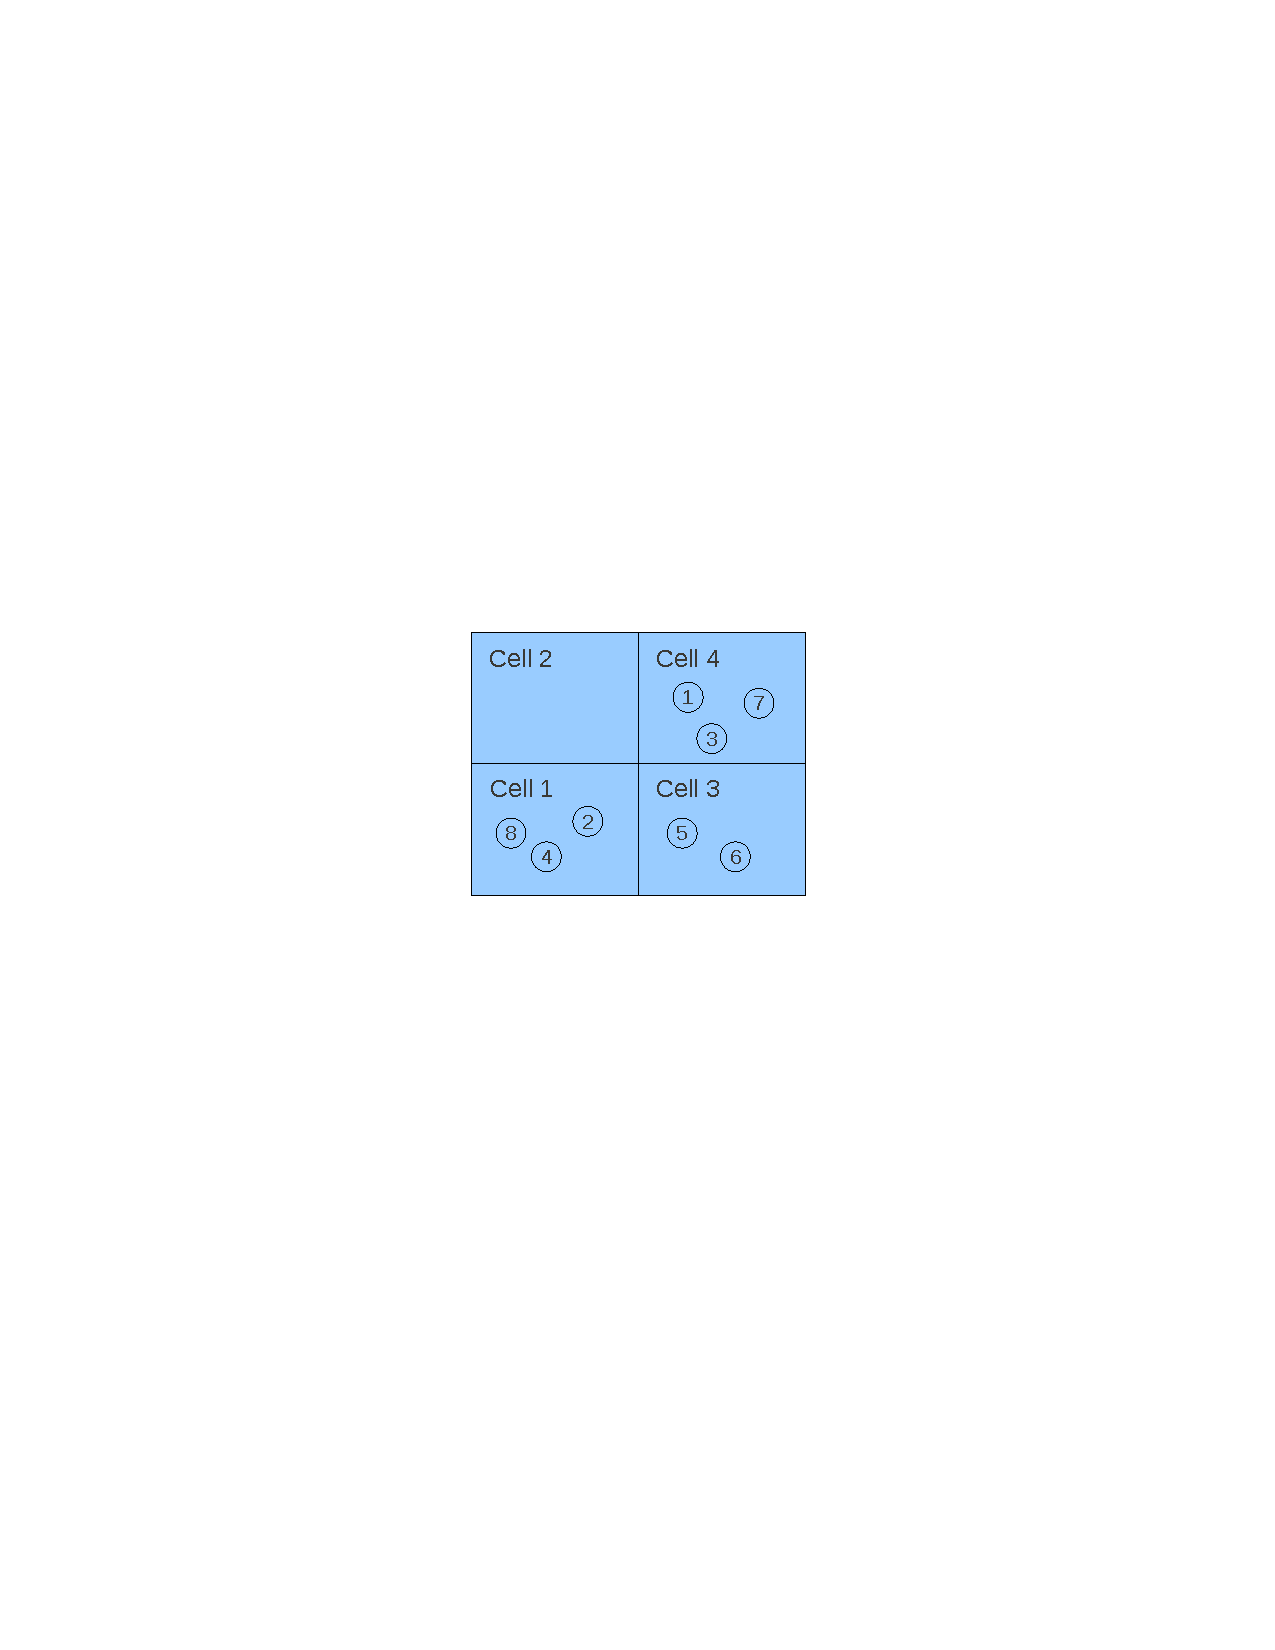
\includegraphics[width=0.4\textwidth]{fig01.pdf}
\caption{\label{ParticleDistribute}各粒子所在网格分布示意图}
\end{figure}


该方法用Head和Link两个一维数组来存储网格和粒子的信息,图\ref{HeadLink}是对应图\ref{ParticleDistribute}的Head和Link数组. Head 中第$i$个元素为第$i$个格子(Cell $i$)中的最大编号粒子的编号,比如第3个格子(Cell 3)中,最大编号的粒子为7, 因此Head中的第3个元素为7. Link中第i个元素表示与i号粒子在同一格子中且比i号粒子编号稍小的一个粒子的编号, 比如Link中第4个元素是2,表示与4号粒子在同一格子中且编号比4号稍少的粒子是2号粒子。

\begin{figure}[!htb]
\centering
\begin{tabular}{lllllllll}
 & 1 & 2 & 3 & 4 &  &  &  &  \\
\cline{2-5}
\multicolumn{1}{l|}{Head} & \multicolumn{1}{l|}{8} & \multicolumn{1}{l|}{0} & \multicolumn{1}{l|}{6} & \multicolumn{1}{l|}{7} &  &  &  &  \\
\cline{2-5}
 & 1 & 2 & 3 & 4 & 5 & 6 & 7 & 8 \\
\cline{2-9}
\multicolumn{1}{l|}{Link} & \multicolumn{1}{l|}{0} & \multicolumn{1}{l|}{0} & \multicolumn{1}{l|}{1} & \multicolumn{1}{l|}{2} & \multicolumn{1}{l|}{0} & \multicolumn{1}{l|}{5} & \multicolumn{1}{l|}{3} & \multicolumn{1}{l|}{4} \\
\cline{2-9}
\end{tabular}
\caption{\label{HeadLink}Head 和Link数组}
\end{figure}

这样,我们就可以通过Head和Link这两个数组来访问某个格子中所有的粒子编号了,比如我们要访问第4个格子中的所有粒子,则具体过程如下:

\begin{enumerate}
\item 先由Head(4) = 7找到第4个格子中最大号粒子即7号粒子
\item 再由Link(7)  = 3找到第4个格子中次大号粒子即3号粒子
\item 再由Link(3)  = 1找到第4个格子中次大号粒子即1号粒子
\item 再由Link(1)  = 0判断第4个格子中没有其它可搜索的粒子
\end{enumerate}

\subsection{Linked-list cells方法的实现}

要应用Linked-list cells方法,首先得根据粒子和网格的信息生成相应的Head和Link数组. 图\ref{Alg1}是生成Link和Head数组的伪代码.

\begin{figure}[!htb]
\centering
\begin{tabular}{|lll|}
\hline
\multicolumn{3}{|l|}{Algorithm 1:  Generate Head and Link arrays} \\
\hline
\multicolumn{3}{|l|}{Initialize Link and Head} \\
\multicolumn{3}{|l|}{Do for all particles i form 1 to n} \\
 &       & Icell = The number of cell which contain  particle i \\
  &       & \\
 &  & \textcolor{blue}{! Link to the previous occupant } \\
 &  &  Link(i) = Head(Icell) \\
   &       & \\
 &  & \textcolor{blue}{! The last one goes to the header } \\
 &  & Head(Icell) = i \\
\multicolumn{3}{|l|}{End do} \\
\hline
\end{tabular}
\caption{\label{Alg1}生成Link和Head数组的伪代码}
\end{figure}

由Algorithm 1生成Link和Head数组后,就可以很方便的访问某个格子中的所有粒子,实现访问的伪代码如图\ref{Alg2}

\begin{figure}[!htb]
\centering
\begin{tabular}{lll}
\hline
\multicolumn{3}{|l|}{Algorithm 2:  Access All Particle in One Cell} \\
\hline
\multicolumn{3}{|l|}{i = Head(Number of one cell)} \\
\multicolumn{3}{|l|}{Do while I not equal 0} \\
\multicolumn{1}{|l}{} &  & \multicolumn{1}{l|}{Access the i-th particle} \\
\multicolumn{1}{|l}{} &  & \multicolumn{1}{l|}{i = Link(i)} \\
\multicolumn{3}{|l|}{End do} \\
\hline
\end{tabular}
\caption{\label{Alg2}访问某一格子中粒子的伪代码}
\end{figure}


\section{Data locality 方法}

Data locality 是一种按照常规的顺序存储各格子中的粒子信息. 如图\ref{Alg3}, 该方法首先需要将所用粒子的序号OldList按照所在格子分好类, 生成新的序列为NewList. 再用CellEnd数组存放每个格子中所有粒子在NewList中的位置, NewList中第CellEnd(i)+1到第CellEnd(i+1)个元素表示第i个格子中的所用粒子. 比如CellEnd(3)+1=4, CellEnd(3+1)=5, 表示NewList中第4到第5个元素表示第3个格子中的粒子序号.

\begin{figure}[!htb]
\centering
\begin{tabular}{lllllllll}
 & 1 & 2 & 3 & 4 & 5 & 6 & 7 & 8 \\
\cline{2-9}
\multicolumn{1}{l|}{OldList} & \multicolumn{1}{l|}{1} & \multicolumn{1}{l|}{2} & \multicolumn{1}{l|}{3} & \multicolumn{1}{l|}{4} & \multicolumn{1}{l|}{5} & \multicolumn{1}{l|}{6} & \multicolumn{1}{l|}{7} & \multicolumn{1}{l|}{8} \\
\cline{2-9}
 & 1 & 2 & 3 & 4 & 5 & 6 & 7 & 8 \\
\cline{2-9}
\multicolumn{1}{l|}{NewList} & \multicolumn{1}{l|}{\textcolor{red}{2}} & \multicolumn{1}{l|}{\textcolor{red}{4}} & \multicolumn{1}{l|}{\textcolor{red}{8}} & \multicolumn{1}{l|}{5} & \multicolumn{1}{l|}{6} & \multicolumn{1}{l|}{\textcolor{blue}{1}} & \multicolumn{1}{l|}{\textcolor{blue}{3}} & \multicolumn{1}{l|}{\textcolor{blue}{7}} \\
\cline{2-9}
 & 1 & 2 & 3 & 4 & 5 &  &  &  \\
\cline{2-6}
\multicolumn{1}{l|}{CellEnd} & \multicolumn{1}{l|}{0} & \multicolumn{1}{l|}{3} & \multicolumn{1}{l|}{3} & \multicolumn{1}{l|}{5} & \multicolumn{1}{l|}{8} &  &  &  \\
\cline{2-6}
\end{tabular}
\caption{\label{Alg3}NewList和CellEnd一维数组}
\end{figure}


\subsection{Data locality 方法的实现}

要应用Data locality方法,首先得根据原粒子列表OldList和所在网格的信息生成相应的NewList 和CellEnd 数组. 图\ref{newlist}是生成NewList 和CellEnd数组的伪代码. 附录A给出了对应图\ref{cell}生成的NewList 和CellEnd 数组Fortran95的程序。


\begin{figure}[!htb]
\centering
\begin{tabular}{lll}
\hline
\multicolumn{3}{|l|}{Algorithm 3:  Generate NewList and CellEnd arrays} \\
\hline
\multicolumn{3}{|l|}{Initialize NewList,  CellEnd and Temp} \\
\multicolumn{3}{|l|}{} \\
\multicolumn{3}{|l|}{\textcolor{blue}{! Generate CellEnd array}} \\
\multicolumn{3}{|l|}{Do for all particles i form 1 to n} \\
\multicolumn{1}{|l}{} &  & \multicolumn{1}{l|}{Icell = The index of cell which contain  particle i} \\
\multicolumn{1}{|l}{} &  & \multicolumn{1}{l|}{CellEnd(Icell+1:end) = CellEnd(Icell+1:end) +1} \\
\multicolumn{3}{|l|}{End do} \\
\multicolumn{3}{|l|}{} \\
\multicolumn{3}{|l|}{\textcolor{blue}{! Generate NewList array}} \\
\multicolumn{3}{|l|}{Temp = CellEnd} \\
\multicolumn{3}{|l|}{Do for all particles i from n to 1} \\
\multicolumn{1}{|l}{} &  & \multicolumn{1}{l|}{Icell = The index of cell which contain  particle i} \\
\multicolumn{1}{|l}{} &  & \multicolumn{1}{l|}{ NewList( Temp(Icell+1) ) = I} \\
\multicolumn{1}{|l}{} &  & \multicolumn{1}{l|}{Temp(Icell+1) = Temp(Icell+1)  - 1} \\
\multicolumn{3}{|l|}{End do} \\
\hline
\end{tabular}
\caption{\label{newlist}生成NewList和CellEnd数组的伪代码}
\end{figure}

由Algorithm 1生成Link和Head数组后,就可以很方便的访问某个格子中的所有粒子,实现的访问伪代码如图\ref{Alg4}.


\begin{figure}[!htb]
\centering
\begin{tabular}{lll}
\hline
\multicolumn{3}{|l|}{Algorithm 4:  Access All Particle in One Cell} \\
\hline
\multicolumn{3}{|l|}{Do for i form CellEnd(c)+1 to CellEnd(c+1)} \\
\multicolumn{1}{|l}{} &  & \multicolumn{1}{l|}{access particle NewList(i)} \\
\multicolumn{3}{|l|}{End do} \\
\hline
\end{tabular}
\caption{\label{Alg4}访问某一格子中粒子的伪代码}
\end{figure}


\section{半邻居网格搜索}


首先我们将粒子所在区域划上网格,如图\ref{cell}.并对网格进行编号。网格的编号索引有两种,
一种是用行列来表示,另一种是用单个下标来索引,如红色粒子所在网格即可表示为02行02列,也可用06号网格来引用.

\begin{figure}[!htb]
\centering
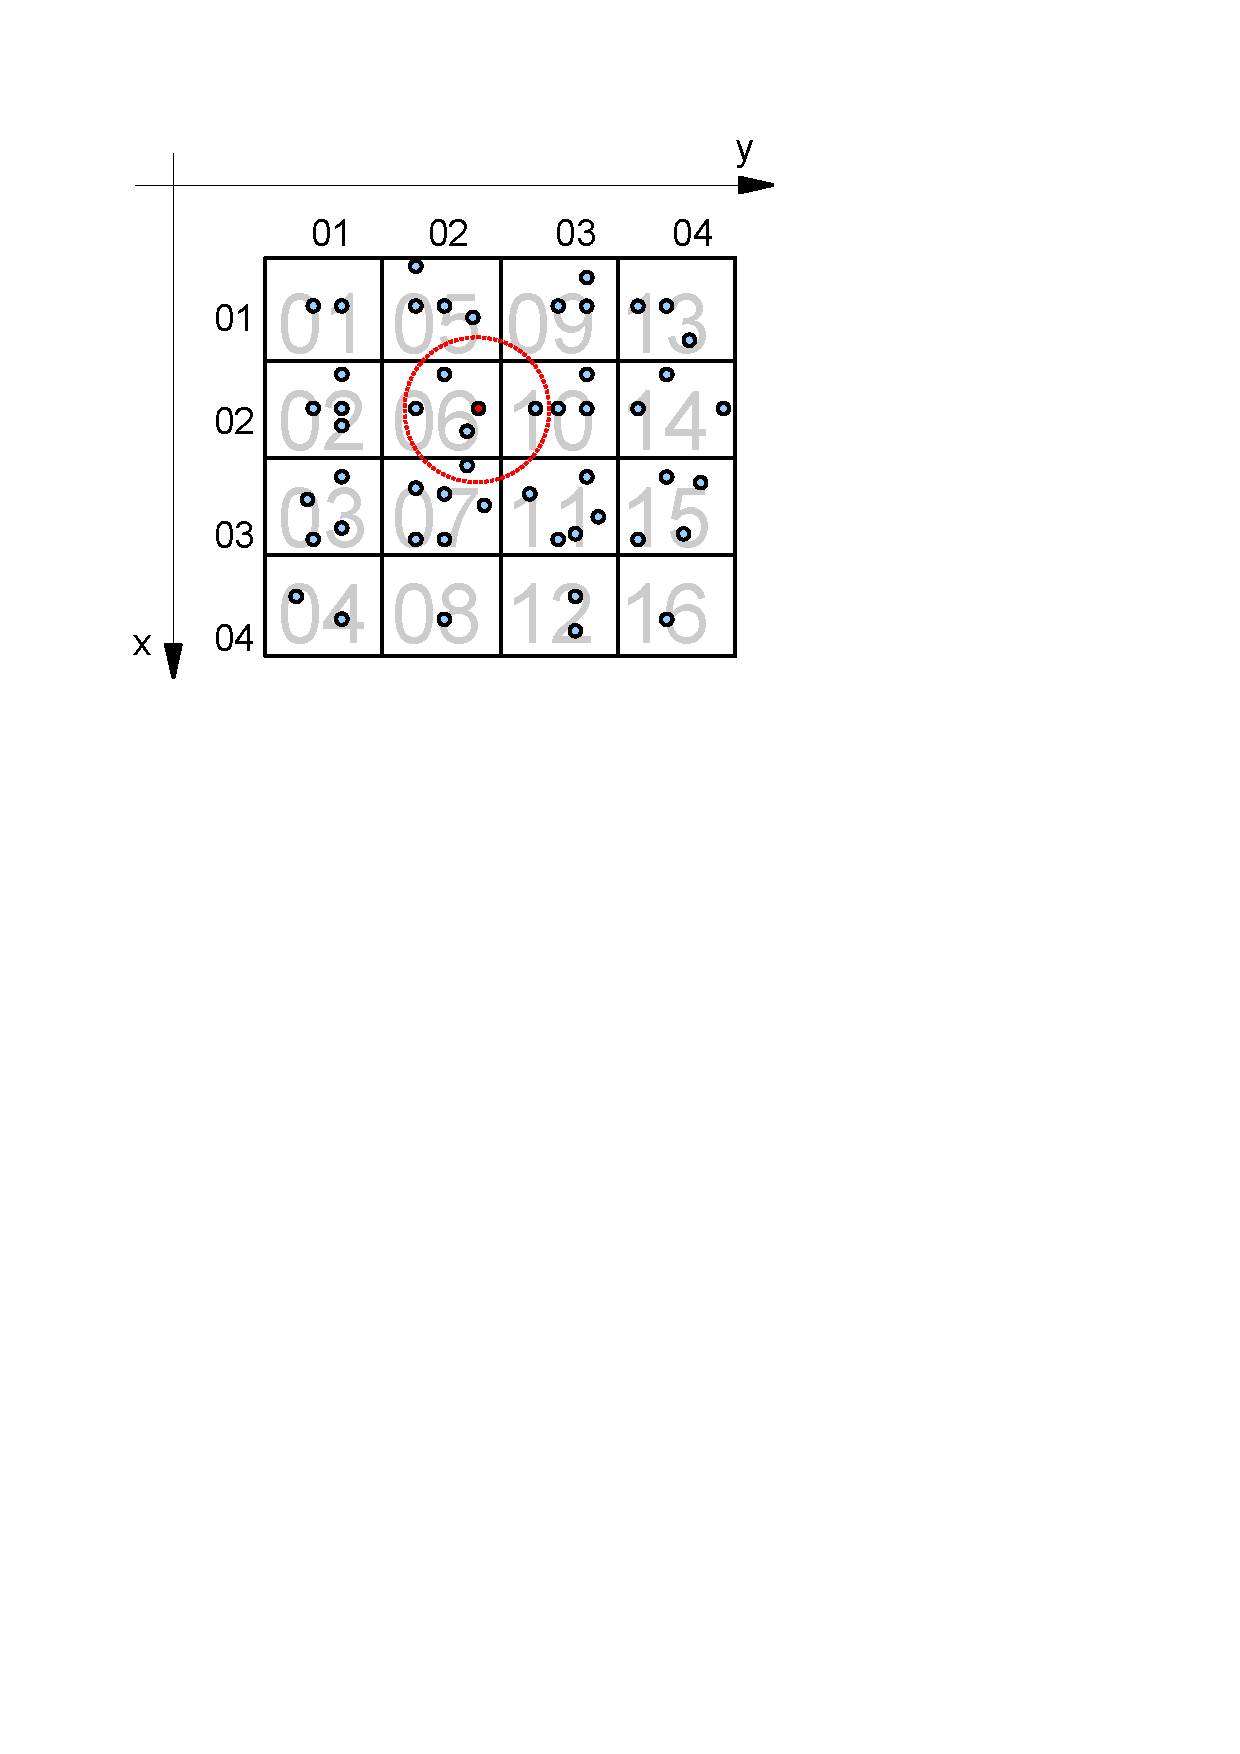
\includegraphics[width=0.5\textwidth]{fig02.pdf}
\caption{\label{cell} 二维空间网格划分示意图}
\end{figure}

我们假设有个$n$粒子,第$i$个粒子空间坐标为$r_i=[x_i, y_i]$, 将所有粒子的坐标存放在以下数组中:
\[
r =\left[
     \begin{array}{c}
       r_1 \\
       r_2 \\
       \vdots \\
       r_n \\
     \end{array}
   \right]=
\left[
\begin{array}{cc}
  x_1 & y_1 \\
  x_2 & y_2 \\
  \vdots & \vdots \\
  x_n & y_n
\end{array}\right]
\]


设空间的大小为$boxl=[L_x,L_y]$; 将空间分成$Nc_x\times Nc_y$个网格,记$N_c=[Nc_x, Nc_y]$, 则第$i$个粒子所在的网格$CellSub_i =[CellSubX_i,CellSubY_j]$为
\[
CellSubX_i = \lfloor\frac{x_i}{Nc_x}\cdot L_x \rfloor + 1, CellSubY_i = \lfloor \frac{y_i}{Nc_y}\cdot L_y \rfloor + 1
\]

其中$\lfloor x\rfloor$ 表示取小于等于$x$的最大整数, 通过下式,我们可以将行列索引转化为单个索引

\[
CellInd_i = CellSubX_i + (CellSubY_i-1)\cdot Nc_x = [CellSubX_i, CellSubY_i -1]\left[
                                                                                \begin{array}{c}
                                                                                  1 \\
                                                                                  Nc_x \\
                                                                                \end{array}
                                                                              \right]
\]

至此,我们可以由每个粒子的坐标位置得到该粒子所在的网格.

由于力的作用是相互的,两个相互作用的粒子间的力是同时的,这使得我们只需要搜索每一个粒子周围一半格子中的粒子,并计算相互作用力. 
图\ref{neighbor}是这种搜索一半网格的示意图,左图为二维情况,只搜索周围8个邻居中的4个及自身,即图中有色的5个格子; 
右图为三维情况, 只搜索周维26个邻居中的13个及自身,即图中画出的格子.


\begin{figure}[!htb]
\centering
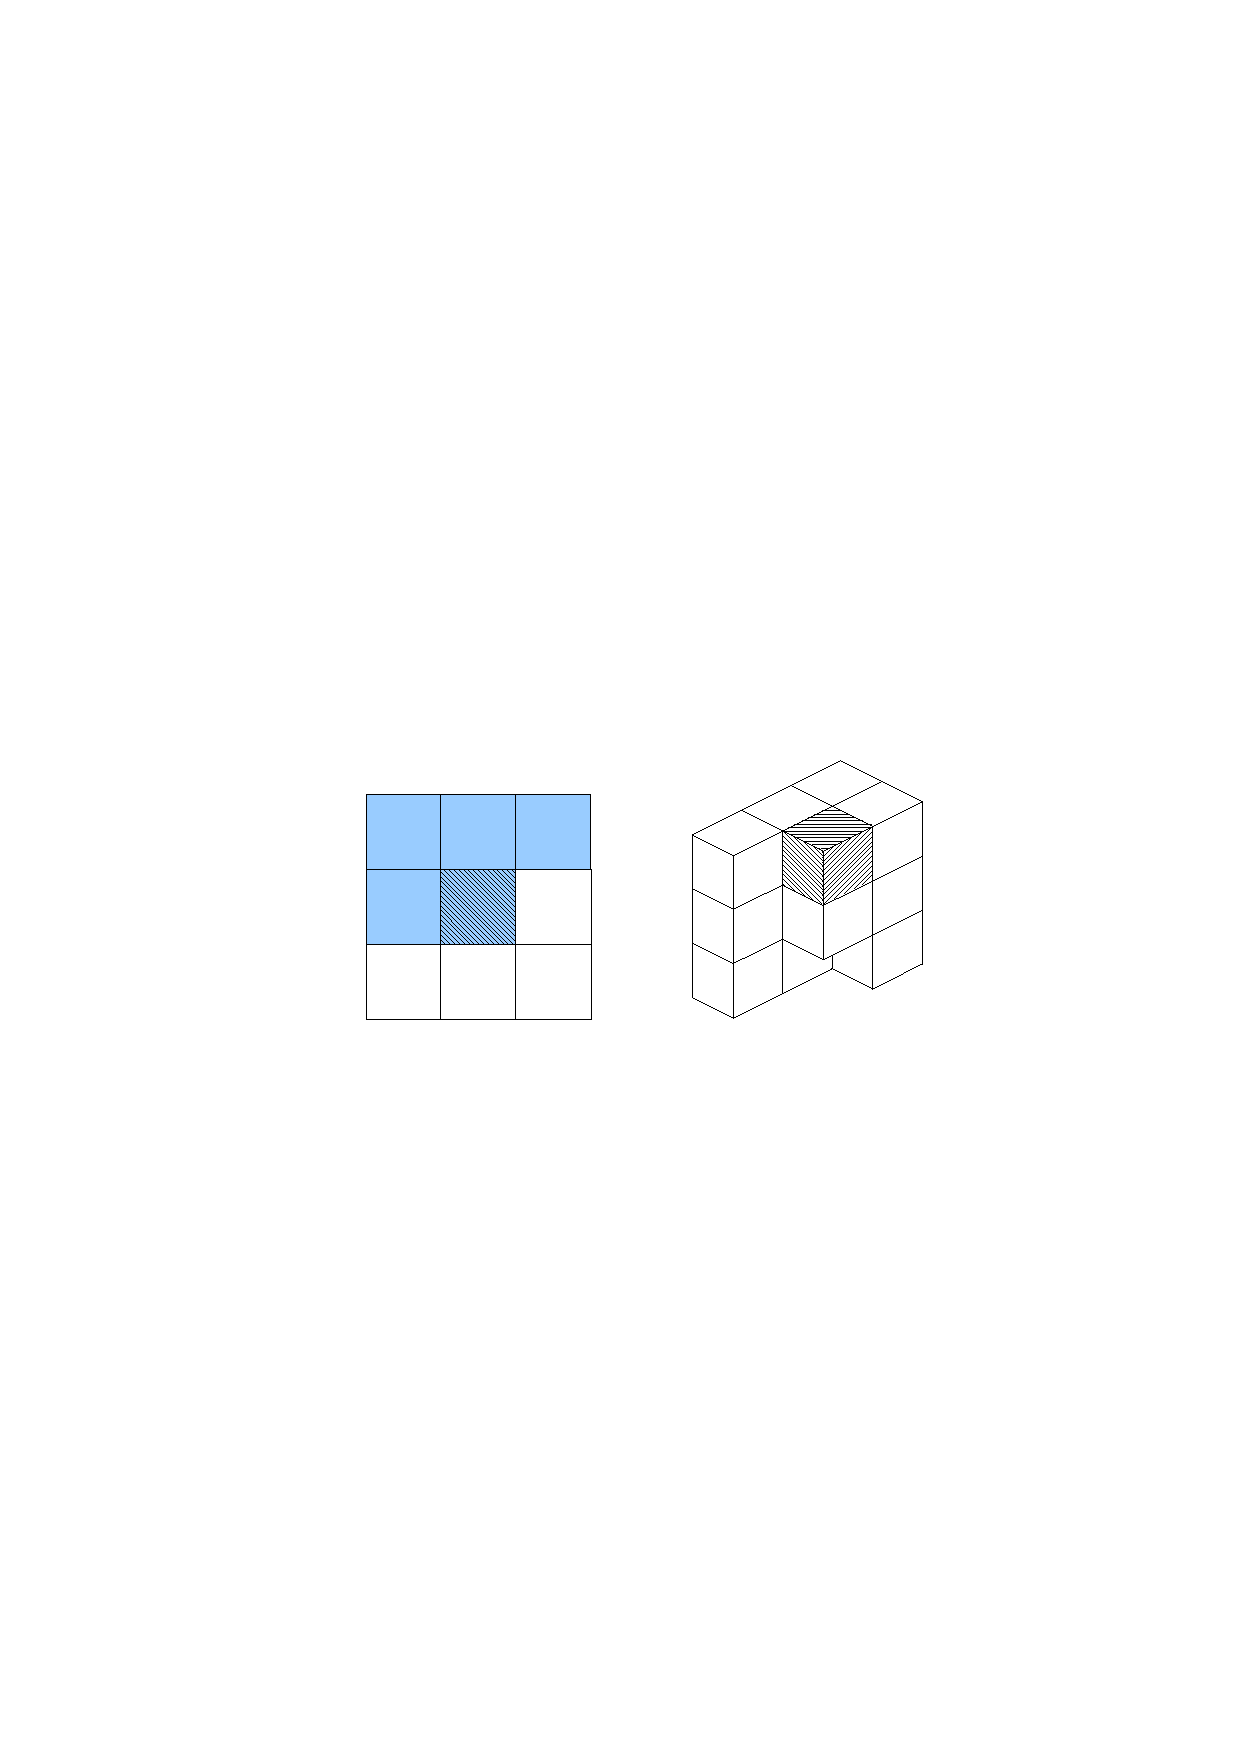
\includegraphics[width=0.6\textwidth]{fig03.pdf}
\caption{\label{neighbor}搜索周围的一半网格示意图(左:二维,右:三维)}
\end{figure}


结合Linked-list cells 和data locality方法,我们可以完成搜索并计算出各粒子间的相互作用力,图\ref{Alg5}给出了结合Linked-list cells方法的搜索过程的伪代码.具体程序见附录B


\begin{figure}[!htb]
\centering
\begin{tabular}{|l|ll|ll|lllll}
\hline
\multicolumn{10}{|l|}{Algorithm 5: half neighbors search base on Linked-list Cells (3D)} \\
\hline
\multicolumn{10}{|l|}{\textbf{Do} for all cells i} \\
 &  & \multicolumn{8}{l|}{CellInd\_i = i} \\
 &  & \multicolumn{8}{l|}{atom\_i = Head(CellInd\_i)} \\
 &  & \multicolumn{8}{l|}{\textcolor{blue}{Do} while atom\_i not equal 0} \\
 &  &  &  & \multicolumn{6}{l|}{\textcolor{red}{Do} for all 14 cells j in the neighborhood of cell i} \\
 &  &  &  &  &  & \multicolumn{4}{l|}{ CellInd\_j = Index of cells j} \\
 &  &  &  &  &  & \multicolumn{4}{l|}{If  CellInd\_i equal CellInd\_j  then} \\
 &  &  &  &  &  &  &  & \multicolumn{2}{l|}{atom\_j = Link(atom\_i)} \\
 &  &  &  &  &  & \multicolumn{4}{l|}{Else} \\
 &  &  &  &  &  &  &  & \multicolumn{2}{l|}{atom\_j = head(CellInd\_j)} \\
 &  &  &  &  &  & \multicolumn{4}{l|}{End if} \\
 &  &  &  &  &  & \multicolumn{4}{l|}{Do while atom\_j not equal 0} \\
 &  &  &  &  &  &  &  & \multicolumn{2}{l|}{\textcolor{blue}{!*******************************************}} \\
 &  &  &  &  &  &  &  & \multicolumn{2}{l|}{compute the force between atom\_i and atom\_j in here} \\
 &  &  &  &  &  &  &  & \multicolumn{2}{l|}{\textcolor{blue}{!*******************************************}} \\
 &  &  &  &  &  &  &  & \multicolumn{2}{l|}{ atom\_j = link(atom\_j)} \\
 &  &  &  &  &  & \multicolumn{4}{l|}{End do} \\
 &  &  &  & \multicolumn{6}{l|}{\textcolor{red}{End do}} \\
 &  &  &  & \multicolumn{6}{l|}{atom\_i = Link(atom\_i)} \\
 &  & \multicolumn{8}{l|}{\textcolor{blue}{End do }} \\
\multicolumn{10}{|l|}{\textbf{End do}} \\
\hline
\end{tabular}
\caption{\label{Alg5}基于 Linked-list cells方法的网格搜索伪代码}
\end{figure}

\newpage

\appendix
\section{Local Data 方法的 NewList\&CellEnd 生成程序举例}

\begin{verbatim}
Program LocalData
!
! Purpose:
!       To generate the NewList and CellEnd array by linked-list cells
!
! Record of revisions:
!       Date            Programmer              Description of change
!       ====            ==========              =====================
!    Nov 1, 2010        Zhou Lvwen                  Original Code
!

implicit none
integer, parameter :: Nc = 4            ! Number of cells
! Cell Index of all atoms or particles
integer, dimension(8) :: CellInd = [4, 1, 4, 1, 3, 3, 4, 1]
integer, dimension(Nc+1) :: CellEnd = 0 ! CellEnd array
integer, dimension(Nc+1) :: Temp = 0    ! A copy of CellEnd for generate NewList
integer, dimension(8) :: NewList = 0    ! NewList array
integer :: i                            ! Loop index
integer :: Icell                        ! Cell index of particle i

do i = 1, 8
   Icell = CellInd(i)
   CellEnd(Icell+1:) = CellEnd(Icell+1:) + 1
end do

Temp = CellEnd

do i = 8, 1, -1
   Icell = CellInd(i)
   NewList( CellEnd(Icell+1) ) = i
   Temp(Icell+1) = Temp(Icell+1) - 1
end do

write(*,'(A, 8(1X,I2), 1X, A)') ' NewList = [', NewList, ']'
write(*,'(A, 5(1X,I2), 1X, A)') ' CellEnd = [', CellEnd, ']'

End program LocalData
\end{verbatim}

\newpage

\section{基于Linked-list cells的网格搜索程序举例}

\begin{verbatim}
Program LinkedList
!
! Purpose:
!       To give An example about half neighbors search base on Linked
!       -list cells
!
! Record of revisions:
!       Date            Programmer              Description of change
!       ====            ==========              =====================
!    Oct 26, 2010       Zhou Lvwen                  Original Code
!


implicit none
integer, parameter :: natom = 100                       ! Number of atoms or particles
integer, dimension(3), parameter :: Nc = [3, 3, 3]      ! Number of cells in x, y and z dimension
real   , dimension(3), parameter :: boxl = [6, 6, 6]    ! Box longth in x, y, and z dimension
real   , dimension(natom,3) :: r                        ! Position of atoms
integer, dimension(natom,3) :: CellSub                  ! Multiple subscripts of cells: atoms
integer, dimension(3) :: CellSub_i, CellSub_j           ! Multiple subscripts of cells: atom i,j
integer, dimension(Nc(1)*Nc(2)*Nc(3)) :: head  = 0      !
integer, dimension(natom) ::  link = 0                  !
integer :: i, j, k, l                                   ! Loop index
integer :: CellInd_i, CellInd_j                         ! Index of cell i,j
integer :: atom_i, atom_j                               ! Index of atom i,j
integer, dimension(14,3) :: Dc                          ! 14 Neighbors of cell(0,0,0)
integer :: sub2ind                                      ! Function: Linear index from
                                                        ! multiple subscripts


! Build neighbor cells list
l = 1
do i = -1, 1
   do j = -1, 1
     do k = -1, 1
        if ((i + j + k)>=0 .and. k >= 0) then
           Dc(l,:) = [i, j, k]
           l = l+1
        end if
     end do
   end do
end do

! Generate the random position of all atoms or particles
do i = 1, 3
   do j = 1, natom
      call random_number(r(j,i))
   end do
end do

! Calculate cell subscript values of all atoms or particles
do i = 1, 3
   r(:, i) = r(:, i) * boxl(i)
   CellSub(:,i) = ceiling( r(:,i)/boxl(i) * Nc(i))
end do

! Generate the link array and head array by linked-list cells
do i = 1, natom
   CellInd_i = sub2ind(Nc, CellSub(i,:))
   write(*,*) CellSub(i,:), CellInd_i
   ! Link to the previous occupant (or EMPTY if you're the 1st)
   link(i) = head(CellInd_i)

   ! The last one goes to the header
   head(CellInd_i) = i
end do



do i = 1, Nc(1)*Nc(2)*Nc(3)
   CellInd_i = i
   atom_i = head(CellInd_i)
   do while (atom_i /= 0)

      do j = 1, 14
         CellSub_j =  CellSub(atom_i,:) + Dc(j,:)

         ! Periodic boundary condition
         do k = 1, 3
            if (CellSub_j(k) <  1    ) CellSub_j(k) = CellSub_j(k) + Nc(k)
            if (CellSub_j(k) >  Nc(k)) CellSub_j(k) = CellSub_j(k) - Nc(k)
         end do

         CellInd_j = sub2ind(Nc, CellSub_j)

         if (CellInd_i == CellInd_j) then
            atom_j = link(atom_i)
         else
            atom_j = head(CellInd_j)
         end if

         do while(atom_j /= 0)
            !*************************************************
            !compute the force between atom_i and atom_j in here
            !
            ! r_ij = r(atom_i,:) - r(atom_j,:)
            !
            !*************************************************
           atom_j = link(atom_j)
         end do
      end do
      atom_i = link(atom_i)
   end do
end do


End program LinkedList

!**************************************************************************************

Integer Function sub2ind(siz,sub)
!
! Purpose:
!       To determine  the equivalent single index corresponding  to a
!       given set of subscript values.
!
!       siz =[siz_x, siz_y, siz_z]   sub = [sub_x, sub_y, sub_z]
!
!                                         /  sub_x  \
!       ind = [siz_x, siz_y-1, siz_z-1] * |  sub_y  |
!                                         \  sub_z  /
! Record of revisions:
!       Date            Programmer              Description of change
!       ====            ==========              =====================
!    Oct 26, 2010        Zhou Lvwen                  Original Code
!

implicit none

integer, intent(in), dimension(3) :: siz	! arrary size
integer, intent(in), dimension(3) :: sub	! subscript value


sub2ind = dot_product(sub-[0,1,1],[1, siz(1), siz(2)*siz(3)])

End function sub2ind
\end{verbatim}
\end{document}
